%==========================================
%
% Sibgrapi 2017 paper
% Example of IEEEtran.cls, adapted for Sibgrapi 2017 
%
%==========================================

% *** Authors should verify (and, if needed, correct) their LaTeX system  ***
% *** with the testflow diagnostic prior to trusting their LaTeX platform ***
% *** with production work. The IEEE's font choices and paper sizes can   ***
% *** trigger bugs that do not appear when using other class files.       ***                          ***
% The testflow support page is at:
% http://www.michaelshell.org/tex/testflow/

\documentclass[10pt,conference]{IEEEtran}


% Some very useful LaTeX packages include:
% (uncomment the ones you want to load)


% *** MISC UTILITY PACKAGES ***
%
%\usepackage{ifpdf}
% Heiko Oberdiek's ifpdf.sty is very useful if you need conditional
% compilation based on whether the output is pdf or dvi.
% usage:
% \ifpdf
%   % pdf code
% \else
%   % dvi code
% \fi
% The latest version of ifpdf.sty can be obtained from:
% http://www.ctan.org/pkg/ifpdf
% Also, note that IEEEtran.cls V1.7 and later provides a builtin
% \ifCLASSINFOpdf conditional that works the same way.
% When switching from latex to pdflatex and vice-versa, the compiler may
% have to be run twice to clear warning/error messages.
% para acentuação
\usepackage[utf8]{inputenc}
\usepackage[brazilian]{babel}



% *** CITATION PACKAGES ***
%
\usepackage{cite}
% cite.sty was written by Donald Arseneau
% V1.6 and later of IEEEtran pre-defines the format of the cite.sty package
% \cite{} output to follow that of the IEEE. Loading the cite package will
% result in citation numbers being automatically sorted and properly
% "compressed/ranged". e.g., [1], [9], [2], [7], [5], [6] without using
% cite.sty will become [1], [2], [5]--[7], [9] using cite.sty. cite.sty's
% \cite will automatically add leading space, if needed. Use cite.sty's
% noadjust option (cite.sty V3.8 and later) if you want to turn this off
% such as if a citation ever needs to be enclosed in parenthesis.
% cite.sty is already installed on most LaTeX systems. Be sure and use
% version 5.0 (2009-03-20) and later if using hyperref.sty.
% The latest version can be obtained at:
% http://www.ctan.org/pkg/cite
% The documentation is contained in the cite.sty file itself.






% *** GRAPHICS RELATED PACKAGES ***
%
\ifCLASSINFOpdf
   \usepackage[pdftex]{graphicx}
  % declare the path(s) where your graphic files are
   \graphicspath{{figs/}}
  % and their extensions so you won't have to specify these with
  % every instance of \includegraphics
   \DeclareGraphicsExtensions{.pdf,.jpeg,.png}
\else
  % or other class option (dvipsone, dvipdf, if not using dvips). graphicx
  % will default to the driver specified in the system graphics.cfg if no
  % driver is specified.
   \usepackage[dvips]{graphicx}
  % declare the path(s) where your graphic files are
   \graphicspath{{../figs/}}
  % and their extensions so you won't have to specify these with
  % every instance of \includegraphics
   \DeclareGraphicsExtensions{.eps}
\fi
% graphicx was written by David Carlisle and Sebastian Rahtz. It is
% required if you want graphics, photos, etc. graphicx.sty is already
% installed on most LaTeX systems. The latest version and documentation
% can be obtained at: 
% http://www.ctan.org/pkg/graphicx
% Another good source of documentation is "Using Imported Graphics in
% LaTeX2e" by Keith Reckdahl which can be found at:
% http://www.ctan.org/pkg/epslatex
%
% latex, and pdflatex in dvi mode, support graphics in encapsulated
% postscript (.eps) format. pdflatex in pdf mode supports graphics
% in .pdf, .jpeg, .png and .mps (metapost) formats. Users should ensure
% that all non-photo figures use a vector format (.eps, .pdf, .mps) and
% not a bitmapped formats (.jpeg, .png). The IEEE frowns on bitmapped formats
% which can result in "jaggedy"/blurry rendering of lines and letters as
% well as large increases in file sizes.
%
% You can find documentation about the pdfTeX application at:
% http://www.tug.org/applications/pdftex





% *** MATH PACKAGES ***
%
\usepackage[cmex10]{amsmath}
% A popular package from the American Mathematical Society that provides
% many useful and powerful commands for dealing with mathematics.
%
% Note that the amsmath package sets \interdisplaylinepenalty to 10000
% thus preventing page breaks from occurring within multiline equations. Use:
\interdisplaylinepenalty=2500
% after loading amsmath to restore such page breaks as IEEEtran.cls normally
% does. amsmath.sty is already installed on most LaTeX systems. The latest
% version and documentation can be obtained at:
% http://www.ctan.org/pkg/amsmath
\usepackage{amsthm}
\newtheorem{definition}{Definition}




% *** SPECIALIZED LIST PACKAGES ***
%
\usepackage{algorithmic}
% algorithmic.sty was written by Peter Williams and Rogerio Brito.
% This package provides an algorithmic environment fo describing algorithms.
% You can use the algorithmic environment in-text or within a figure
% environment to provide for a floating algorithm. Do NOT use the algorithm
% floating environment provided by algorithm.sty (by the same authors) or
% algorithm2e.sty (by Christophe Fiorio) as the IEEE does not use dedicated
% algorithm float types and packages that provide these will not provide
% correct IEEE style captions. The latest version and documentation of
% algorithmic.sty can be obtained at:
% http://www.ctan.org/pkg/algorithms
% Also of interest may be the (relatively newer and more customizable)
% algorithmicx.sty package by Szasz Janos:
% http://www.ctan.org/pkg/algorithmicx




% *** ALIGNMENT PACKAGES ***
%
\usepackage{array}
% Frank Mittelbach's and David Carlisle's array.sty patches and improves
% the standard LaTeX2e array and tabular environments to provide better
% appearance and additional user controls. As the default LaTeX2e table
% generation code is lacking to the point of almost being broken with
% respect to the quality of the end results, all users are strongly
% advised to use an enhanced (at the very least that provided by array.sty)
% set of table tools. array.sty is already installed on most systems. The
% latest version and documentation can be obtained at:
% http://www.ctan.org/pkg/array


% IEEEtran contains the IEEEeqnarray family of commands that can be used to
% generate multiline equations as well as matrices, tables, etc., of high
% quality.




% *** SUBFIGURE PACKAGES ***
\ifCLASSOPTIONcompsoc
  \usepackage[caption=false,font=normalsize,labelfont=sf,textfont=sf]{subfig}
\else
  \usepackage[caption=false,font=footnotesize]{subfig}
\fi
% subfig.sty, written by Steven Douglas Cochran, is the modern replacement
% for subfigure.sty, the latter of which is no longer maintained and is
% incompatible with some LaTeX packages including fixltx2e. However,
% subfig.sty requires and automatically loads Axel Sommerfeldt's caption.sty
% which will override IEEEtran.cls' handling of captions and this will result
% in non-IEEE style figure/table captions. To prevent this problem, be sure
% and invoke subfig.sty's "caption=false" package option (available since
% subfig.sty version 1.3, 2005/06/28) as this is will preserve IEEEtran.cls
% handling of captions.
% Note that the Computer Society format requires a larger sans serif font
% than the serif footnote size font used in traditional IEEE formatting
% and thus the need to invoke different subfig.sty package options depending
% on whether compsoc mode has been enabled.
%
% The latest version and documentation of subfig.sty can be obtained at:
% http://www.ctan.org/pkg/subfig




% *** FLOAT PACKAGES ***
%
%\usepackage{fixltx2e}
% fixltx2e, the successor to the earlier fix2col.sty, was written by
% Frank Mittelbach and David Carlisle. This package corrects a few problems
% in the LaTeX2e kernel, the most notable of which is that in current
% LaTeX2e releases, the ordering of single and double column floats is not
% guaranteed to be preserved. Thus, an unpatched LaTeX2e can allow a
% single column figure to be placed prior to an earlier double column
% figure.
% Be aware that LaTeX2e kernels dated 2015 and later have fixltx2e.sty's
% corrections already built into the system in which case a warning will
% be issued if an attempt is made to load fixltx2e.sty as it is no longer
% needed.
% The latest version and documentation can be found at:
% http://www.ctan.org/pkg/fixltx2e


%\usepackage{stfloats}
% stfloats.sty was written by Sigitas Tolusis. This package gives LaTeX2e
% the ability to do double column floats at the bottom of the page as well
% as the top. (e.g., "\begin{figure*}[!b]" is not normally possible in
% LaTeX2e). It also provides a command:
%\fnbelowfloat
% to enable the placement of footnotes below bottom floats (the standard
% LaTeX2e kernel puts them above bottom floats). This is an invasive package
% which rewrites many portions of the LaTeX2e float routines. It may not work
% with other packages that modify the LaTeX2e float routines. The latest
% version and documentation can be obtained at:
% http://www.ctan.org/pkg/stfloats
% Do not use the stfloats baselinefloat ability as the IEEE does not allow
% \baselineskip to stretch. Authors submitting work to the IEEE should note
% that the IEEE rarely uses double column equations and that authors should try
% to avoid such use. Do not be tempted to use the cuted.sty or midfloat.sty
% packages (also by Sigitas Tolusis) as the IEEE does not format its papers in
% such ways.
% Do not attempt to use stfloats with fixltx2e as they are incompatible.
% Instead, use Morten Hogholm'a dblfloatfix which combines the features
% of both fixltx2e and stfloats:
%
% \usepackage{dblfloatfix}
% The latest version can be found at:
% http://www.ctan.org/pkg/dblfloatfix




% *** PDF, URL AND HYPERLINK PACKAGES ***
%
\usepackage{url}
% url.sty was written by Donald Arseneau. It provides better support for
% handling and breaking URLs. url.sty is already installed on most LaTeX
% systems. The latest version and documentation can be obtained at:
% http://www.ctan.org/pkg/url
% Basically, \url{my_url_here}.




% *** Do not adjust lengths that control margins, column widths, etc. ***
% *** Do not use packages that alter fonts (such as pslatex).         ***
% There should be no need to do such things with IEEEtran.cls V1.6 and later.
% (Unless specifically asked to do so by the journal or conference you plan
% to submit to, of course. )


% correct bad hyphenation here
\hyphenation{op-tical net-works semi-conduc-tor}


\begin{document}
%
% paper title
% Titles are generally capitalized except for words such as a, an, and, as,
% at, but, by, for, in, nor, of, on, or, the, to and up, which are usually
% not capitalized unless they are the first or last word of the title.
% Linebreaks \\ can be used within to get better formatting as desired.
% Do not put math or special symbols in the title.
\title{Um Sistema Visual para Análise Personalizada da Segurança em Cidades}

%------------------------------------------------------------------------- 
% change the % on next lines to produce the final camera-ready version 
\newif\iffinal
%\finalfalse
\finaltrue
% Id do paper enviado para o SIBGRAPI
\newcommand{\jemsid}{99999}
%------------------------------------------------------------------------- 

% author names and affiliations
% use a multiple column layout for up to two different
% affiliations

\iffinal

% author names and affiliations
% use a multiple column layout for up to three different
% affiliations
\author{\IEEEauthorblockN{Rafael Heitor Correia de Melo e Ícaro Goulart Faria Motta França}
\IEEEauthorblockA{Instituto de Computação\\
Universidade Federal Fluminense (UFF)\\
Niterói, RJ, Brazil\\
Email: \{rmelo,igoulart\}@ic.uff.br}}

% conference papers do not typically use \thanks and this command
% is locked out in conference mode. If really needed, such as for
% the acknowledgment of grants, issue a \IEEEoverridecommandlockouts
% after \documentclass

% for over three affiliations, or if they all won't fit within the width
% of the page, use this alternative format:
% 
%\author{\IEEEauthorblockN{Michael Shell\IEEEauthorrefmark{1},
%Homer Simpson\IEEEauthorrefmark{2},
%James Kirk\IEEEauthorrefmark{3}, 
%Montgomery Scott\IEEEauthorrefmark{3} and
%Eldon Tyrell\IEEEauthorrefmark{4}}
%\IEEEauthorblockA{\IEEEauthorrefmark{1}School of Electrical and Computer Engineering\\
%Georgia Institute of Technology,
%Atlanta, Georgia 30332--0250\\ Email: see http://www.michaelshell.org/contact.html}
%\IEEEauthorblockA{\IEEEauthorrefmark{2}Twentieth Century Fox, Springfield, USA\\
%Email: homer@thesimpsons.com}
%\IEEEauthorblockA{\IEEEauthorrefmark{3}Starfleet Academy, San Francisco, California 96678-2391\\
%Telephone: (800) 555--1212, Fax: (888) 555--1212}
%\IEEEauthorblockA{\IEEEauthorrefmark{4}Tyrell Inc., 123 Replicant Street, Los Angeles, California 90210--4321}}

\else
  \author{Sibgrapi paper ID: \jemsid \\ }
\fi


% make the title area
\maketitle

% As a general rule, do not put math, special symbols or citations
% in the abstract
\begin{abstract}
Neste trabalho descrevemos a criação de um sistema visual interativo para auxílio no entendimento de dados de segurança de cidades. Utilizamos mapas e gráficos que interagem entre si e com uma a configuração personalizada. O objetivo principal é permitir o entendimento da saturação de áreas em relação a crimes e atuação policial bem como buscar relações entre estes dois indicadores. Algumas análises geraram resultados não óbvios como a presença de municípios do interior e região dos lagos com os mais altos índices de violência por habitante.
\end{abstract}

% no keywords




% For peerreview papers, this IEEEtran command inserts a page break and
% creates the second title. It will be ignored for other modes.
\IEEEpeerreviewmaketitle



\section{Introdução}

O grande uso de dispositivos inteligentes vem alavancando a geração de dados numa velocidade e quantidade maior do que a capacidade de processamento sobre estes dados para geração de informação. Junto com esta tendência as grandes cidades tem cada vez mais feito investimentos no sentido de se tornarem cidades inteligentes. Pesquisadores como Cohen em \cite{EXAME.COM2015} definem cidades inteligentes como as que conseguem se desenvolver economicamente ao mesmo tempo que aumentam a qualidade de vida dos habitantes ao gerar eficiência nas operações urbanas. Uma forma de aumentar a eficiência das operações urbanas e a facilitação no acesso a informações o que pode ser feito através de sistemas de visualização de dados.

A partir dos dados esparsos existentes e cada vez mais disponibilizados pelas cidades e seus habitantes através do extenso uso de redes sociais ou aplicativos colaborativos não é fácil se obter informações, mesmo que ela esteja presentes nestes dados. A construção de um sistema de visualização para fins específicos e voltados para as necessidades de obtenção de informação vem emergindo como uma grande área de pesquisa nos últimos anos.

Neste trabalho focamos na construção de um sistema interativo de visualização sobre os dados de segurança do estado do Rio de Janeiro com o intuito de permitir o entendimento da saturação de áreas em relação a crimes e atuação policial bem como buscar relações entre estes dois indicadores. Esta ferramenta pode servir tanto para a população em geral como para seguradoras, imobiliárias enfim todo e qualquer indivíduo ou grupo que sentir necessidade de quantificar a ocorrência de eventos que tenham alguma relação com o seu negócio ou ainda algum interesse pessoal.

O restante deste trabalho é apresentado da seguinte forma: A seção 2 descreve o problema; A seção 3 apresenta a nossa proposta de sistema de visualização. Na seção 4 mostramos alguns dos resultados que obtivemos com o uso do sistema. A seção 5 discute a solução e os resultados que podemos obter. Por fim a conclusão e alternativas para trabalhos futuros são apresentadas na seção 6.

\section{Problema}

O crescimento do sentimento de insegurança que assola os moradores do Rio de Janeiro é algo fortemente influenciado pelos canais de comunicação. As informações exibidas nestes canais podem conter viés uma vez que muitas vezes são exibidas informações pontuais na forma de indicadores. Isto acontece até mesmo pelo espaço ou tempo que se tem para veicular uma noticia fazendo com que, por exemplo, se olhe somente para um pequeno conjunto de características e se gere uma conclusão sobre o todo.

A construção e disponibilização de sistemas de visualização “arma” o individuo com a informação permitindo a ele explorar os dados de forma interativa e iterativa. Desta forma cada pessoa pode investigar os dados segundo suas premissas e gerar suas próprias conclusões sobre eles.

Neste trabalho utilizamos os dados disponibilizados pelo ISPDados \cite{ISP2017}, página de dados abertos do Instituto de Segurança Pública (ISP) do Governo do Estado do Rio de Janeiro. Os dados são em termos de quantidades de ocorrências de eventos mensais (intervalo de janeiro de 2013 até março de 2017) para um conjunto de crimes (ex. Homicídios e tentativas, Roubos e Furtos de: residência, veículo, pedestre, carga, coletivo, banco; Estupro dentre outros) e um conjunto de dados de atuações policiais (ex. Apreensões: drogas, armas, menores, prisões; Recuperação de veículos) bem como o número total de ocorrências. Estes dados são distribuídos por circunscrição de delegacia no estado do Rio de Janeiro. Também foram usados os dados da população por município e por circunscrição de delegacia obtidos nesta mesma fonte para permitir o cálculo do valor absoluto (quantidade “crua”) e o valor relativo (quantidade por número de habitantes), para tal consideramos a estimativa de população de 2016. 

\section{Sistema proposto}

Para construção do sistema visual de análise personalizada da segurança em cidades utilizamos \textit{Bootstrap} \cite{Bootstrap2017} para a interface web e configuração dos parâmetros, \textit{Google Maps} \cite{Google2017} para exibição e interação no mapa, D3.js \cite{MikeBostock2017} para construção e interação com os gráficos, \textit{JQuery} \cite{JQuery2017} para tratar eventos de interface. 

Os dados foram obtidos em formato xls (Excel), um para cada evento (crime, ação policial ou registro de ocorrência) e um para cada ano. Os arquivos foram convertidos para o formato CSV removendo colunas e linhas de cabeçalho desnecessárias. Estes arquivos foram então lidos pelo sistema e transformados num dicionário onde a chave é o identificador da Delegacia (DP) e o valor é um objeto contendo os atributos: município, risp (identificador de grande área), aisp (identificador de batalhão) e os três tipos de eventos (crime, número de ocorrências e reações policiais). Cada objeto contém um outro dicionário chamado anos, onde cada ano possui um \textit{array} contendo as contagens dos eventos de cada tipo. Cada evento traz um \textit{array} com a quantidade de cada mês e um adicional com o somatório do ano. Esse dicionário fica na memória, com isso as consultas são realizadas em menos de 1 segundo.

Construímos uma interface de configuração para permitir que sejam definidos os seguintes parâmetros:

\begin{itemize}
\item \textbf{Granularidade} de agregação do tempo (valores possíveis: mês e ano).
\item \textbf{Janela de tempo} que pode ser específica, definindo um intervalo dos itens devidamente agregados segundo a granularidade, ou periódica, definindo os meses e/ou anos a serem analisados. 
\item \textbf{Tabela de pesos} definida para cada tipo de evento (os tipos compreendem o número de registros de ocorrências, o conjunto de eventos relacionados aos crimes e o conjunto relacionado à ação policial). Cada ocorrência pode também ser marcada para ser visualizada ou não.

\item \textbf{Média na série temporal} que determina se a média do índice para todas as regiões será exibida ou não na série temporal.
\end{itemize}

A associação de pesos a cada evento permite ao usuário da análise a criação de índices de violência e de resposta a violência  ponderando os eventos que ele considerar mais relevantes.

Inicialmente é apresentada uma visão geral da quantificação da violência usando o mapa do estado do Rio de Janeiro. As informações de quantidade de eventos foram agrupados por tipos (crimes, atuação policial ou total de registros de ocorrência) e  exibidos no mapa de acordo com as cores via \textit{choropleth}. Foram utilizados grupos de cores definidos em \cite{CynthiaBrewer2013}. Escolhemos um conjunto de cores para cada tipo de evento visando melhorar a identificação visual com a variação das cores no mapa. A visualização deste mapa possibilita a extração direta de informação a respeito de quais as regiões mais afetadas por cada índice de violência/resposta a violência criado. Um exemplo de mapa pode ser visto na figura~\ref{fig_mapaBPM} e a respectiva legenda ao clicar sobre a região referente ao sétimo batalhão pode ser visto na figura~\ref{fig_mapaBPM_legenda}.

\begin{figure}[!t]
\centering
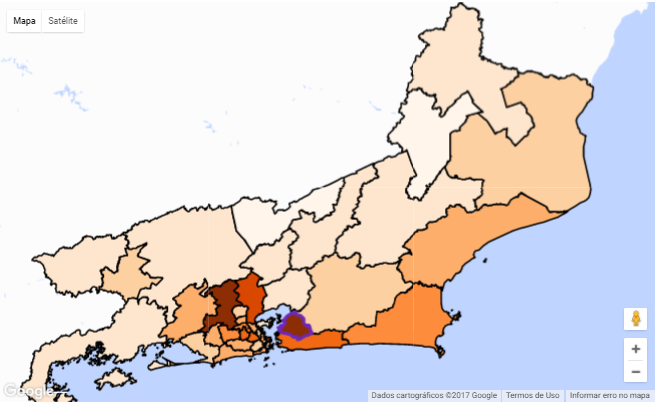
\includegraphics[width=2.5in]{mapa_zoom_batalhao_evento_registros_ocorrencia_bpm_7_municipio_sao_goncalo.png}
% where an .eps filename suffix will be assumed under latex, 
% and a .pdf suffix will be assumed for pdflatex; or what has been declared
% via \DeclareGraphicsExtensions.
\caption{Mapa configurado para zoom = batalhão, tipo de evento = registros de ocorrência e quantificação absoluta com o sétimo batalhão selecionado.}
\label{fig_mapaBPM}
\end{figure}

\begin{figure}[!t]
\centering
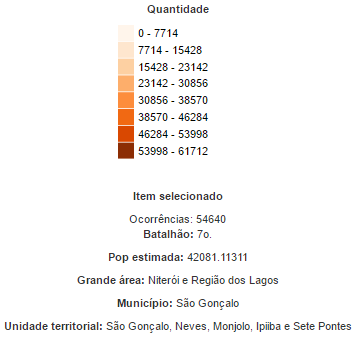
\includegraphics[width=2.5in]{legenda_mapa_zoom_batalhao_evento_registros_ocorrencia_bpm_7_municipio_sao_goncalo.png}
% where an .eps filename suffix will be assumed under latex, 
% and a .pdf suffix will be assumed for pdflatex; or what has been declared
% via \DeclareGraphicsExtensions.
\caption{Legenda do mapa da figura~\ref{fig_mapaBPM}.}
\label{fig_mapaBPM_legenda}
\end{figure}


No mapa permitimos a parametrização da visualização através das seguintes opções:
\begin{itemize}
\item \textbf{Zoom} para determinar os limites territoriais (podendo ser visualizado por Grandes áreas, Batalhão, Município ou Delegacia).
\item \textbf{Tipo do dado} que corresponde ao índice de violência e de resposta configurados na tabela de pesos (separadamente por Crimes, o Total de Ocorrências e as Resposta policiais).
\item \textbf{Quantificação} serve para determinar se o resultado é mostrado de forma "crua" (somente a soma ponderada dos elementos) ou relativa (dividindo o índice anterior pelo tamanho da população e normalizando esta pela região com o maior valor).
\end{itemize} 

Ao clicar sobre uma região no mapa, os dados específicos desta região são exibidos a direita, para uma rápida consulta. Abaixo do mapa, mostramos os gráficos com o histórico de cada indicador, exibidos em três séries temporais (uma para cada tipo de evento). Com isto é possível buscar relações diretas entre os índices de crimes e de atuação policial. Ao lado de cada série temporal, há um gráfico de barras que detalha a quantidade de cada evento por região selecionada. Este gráfico também apresenta o total (soma da quantidade de todos os eventos). Isto serve para identificar quais dos eventos selecionados tem maior impacto sobre os valores totais de cada região.

O sistema possibilita a seleção de mais de uma região do mapa através do clique sobre estas. As séries temporais exibem uma curva para cada região selecionada, permitindo a comparação dos índices criados para cada região e a média para os valores de todas as regiões. 

Seleções em intervalos de qualquer uma das séries temporais ressaltam o intervalo selecionado em todas as três séries para facilitar a busca de correlações.

No gráfico de barras, mostramos em detalhe a quantidade de cada evento por região selecionada. Caso todos os crimes (19 eventos distintos) sejam selecionados, há a necessidade de usar uma paleta de cores com pelo menos 20 cores (19 de crimes mais o total) distintas entre si para diferenciar cada evento. ColorBrewer \cite{CynthiaBrewer2013} fornece no máximo 12 cores distintas. Portanto, usamos a paleta de cores fornecida pelo site pessoal do designer Sasha Trubetskoy \cite{SashaTrubetskoy2017}, onde é definida uma paleta com 20 cores, mais as cores preta e branca.

\section{Resultados e discussão}

Concentramos nossas análises no Zoom por batalhão e por município. Isto por que temos somente os dados de população destas regiões o que nos permite não só fazer uma análise de números absolutos como também uma análise relativa ao tamanho da população. Sempre que falarmos de índices e/ou percentuais estamos falando do índice relativo a população.

Nos resultados apresentados nesta seção, mantivemos todos os pesos com valores iguais. Para os cálculos dos valores relativos fizemos a divisão da quantidade de ocorrências pelo tamanho da população obtendo o índice por habitante. Posteriormente foi feita uma normalização deste índice para o intervalo de 0 a 100 considerando como 100 o valor da região com maior índice. 

A tabela~\ref{table_result_crimes_geral} ilustra os municípios com índices relativos de violência mais altos considerando todos os crimes. O Rio de janeiro apesar de ser a região com mais ocorrências em números absolutos com 696.111 ocorrências ela só apresenta 76\% do índice por habitante em relação a Nilópolis. A nossa hipótese era de que os "campeões" deste índice de violência estariam localizados na capital ou na baixada fluminense. Os resultados mostraram que municípios do interior do estado e região dos lagos como Miguel Pereira, Búzios e Italva também apresentam forte incidência de violência por habitante.

\begin{table}[]
%% increase table row spacing, adjust to taste
\renewcommand{\arraystretch}{1.3}
% if using array.sty, it might be a good idea to tweak the value of
% \extrarowheight as needed to properly center the text within the cells
\caption{Resultado relativo para todos os eventos de crimes}
\label{table_result_crimes_geral}
\centering
%% Some packages, such as MDW tools, offer better commands for making tables
%% than the plain LaTeX2e tabular which is used here.
\begin{tabular}{|c|c|c|}
\hline
\textbf{Município} & \textbf{Valor relativo} & \textbf{Valor absoluto} \\
\hline
Nilópolis & 100 & 22343\\
\hline
Miguel Pereira & 91 & 3186\\
\hline
Buzios & 84 & 3760\\
\hline
São João de Meriti & 83 & 54126\\
\hline
Mesquita & 83 & 20013\\
\hline
Italva & 83 & 1716\\
\hline
Niterói & 82 & 57950\\
\hline
\end{tabular}
\end{table}

Numa consulta semelhante a anterior, mas agora considerando todos os eventos de ações policiais o resultado também foi diferente do esperado. O município de Itatiaia se destacou no índice relativo, sendo seguido de muito longe pelo segundo município (Miracema) que apresentou somente 39\% do seu valor. Ao analisar o gráfico de barras da contagem absoluta de eventos selecionando a região de Itatiaia observamos que o evento que impacta neste índice é a apreensão de drogas (barra verde) como pode ser visto na figura~\ref{fig_barraDrogasItatiaia}.

\begin{figure}[!t]
\centering
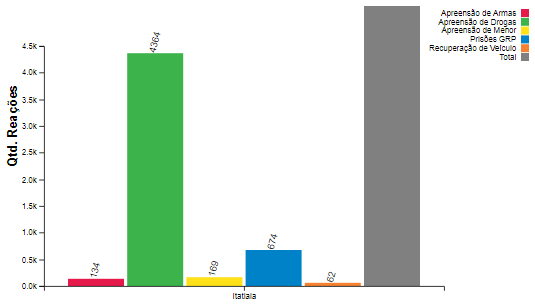
\includegraphics[width=3.5in]{acaoPolicialDrogasItatiaia.png}
\caption{Gráfico de barras do município de Itatiaia, tipo de evento = ação policial (apreensão de drogas e apreensão de armas).}
\label{fig_barraDrogasItatiaia}
\end{figure}

Em relação ao número de registros de ocorrência Búzios, Itatiaia e Miguel Pereira também figuram nas primeiras posições relativas.

Em análises que fizemos no Zoom de batalhão, o sétimo batalhão (São Gonçalo) se destaca no índice geral relativo para todos os eventos em todos os tipos. Considerando somente as ações policiais referentes à apreensão de armas e drogas o quinto batalhão (grande parte do centro, Lapa e Santa Teresa) lidera o índice (na frente do batalhão de São Gonçalo), o que é esperado por conta deste batalhão atender áreas mais boemias. Itatiaia se destaca neste índice relativo quando fazemos a análise por município o que já havia sido observado na análise feita e demonstrada na figura~\ref{fig_barraDrogasItatiaia}. 

Em relação aos roubos a bancos o quarto batalhão (centro e parte da zona norte) encabeça o índice, seguido com uma boa distância pelo quinto batalhão (67\%) no índice relativo. No zoom de município o roubo a banco é liderado por Quissamã, o segundo colocado tem menos de 30\% do seu índice. O curioso é que Quissamã apresenta somente 3 ocorrências no intervalo analisado (2013 até 2017), mas, como número de roubos a banco no geral é baixo, o índice relativo desta região se destaca.

Considerando somente os crimes mais violentos (estupros, homicídios e latrocínio) os municípios que apresentam os piores índices relativos são respectivamente Miguel Pereira, Silva Jardim, Quissamã e Paraty. A figura~\ref{fig_mapaCrimesViolentos} mostra o mapa colorido pelo índice de crime citado. Pelo gráfico de barras da figura~\ref{fig_barraCrimesViolentosMunicipios} podemos observar que cada município apresenta um padrão distinto. Em Miguel Pereira o evento mais relevante é o estupro, já em Silva Jardim o principal é o homicídio culposo, Paraty apresenta grandes quantidades de estupro e homicídio doloso  e Quissamã apresenta equilíbrio entre a quantidade de homicídios e estupro. Todos os municípios apresentam baixas quantidades de latrocínio.

\begin{figure}[!t]
\centering
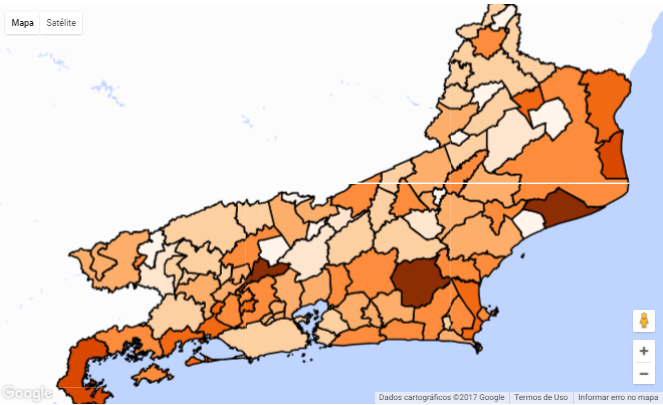
\includegraphics[width=2.5in]{mapaCrimesViolentos.png}
% where an .eps filename suffix will be assumed under latex, 
% and a .pdf suffix will be assumed for pdflatex; or what has been declared
% via \DeclareGraphicsExtensions.
\caption{Mapa configurado para zoom = município, tipo de evento = crimes (estupros, homicídios e latrocínio) e quantificacão relativa.}
\label{fig_mapaCrimesViolentos}
\end{figure}

\begin{figure}[!t]
\centering
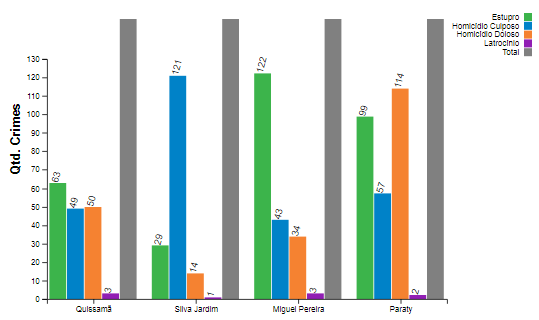
\includegraphics[width=2.5in]{crimesViolentosBarrasMaioresIndices.png}
\caption{Gráfico de barras com municípios de pior índice, tipo de evento = crimes mais violentos (estupro, homicídios e latrocínio).}
\label{fig_barraCrimesViolentosMunicipios}
\end{figure}

Os índices relativos de ações policiais levando em conta somente prisões tem como municípios com valores mais altos: Búzios, Porto Real, Itatiaia e Piraí.

Numa análise da série histórica das prisões observamos uma subida na média a partir de 2015 que é fortemente influenciada pelo aumento da média apresentada nos dados do Rio de Janeiro como pode ser visto na figura~\ref{fig_temporalPrisoes}.

\begin{figure}[!t]
\centering
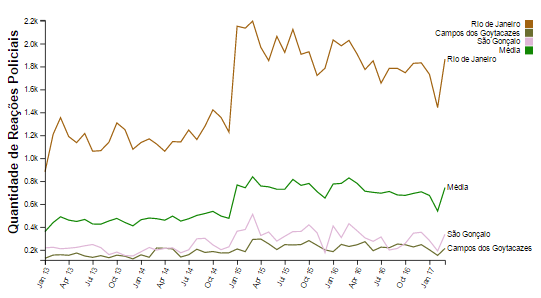
\includegraphics[width=3.5in]{serieTemporalPrisoesPorMunicipio.png}
% where an .eps filename suffix will be assumed under latex, 
% and a .pdf suffix will be assumed for pdflatex; or what has been declared
% via \DeclareGraphicsExtensions.
\caption{Histórico de prisões por município.}
\label{fig_temporalPrisoes}
\end{figure}

Buscando relações entre índices de crimes e atuações policiais consideramos somente os roubos e furtos de veículos e sua recuperação. O gráfico que ilustra a relação direta no histórico considerando o município de São Gonçalo pode ser visto na figura~\ref{fig_relacaoVeiculos}. Selecionamos o intervalo central que separa bem as tendências destes dados em três momentos. O momento inicial (que corresponde ao ano de 2013) onde existe uma tendência de subida nos crimes, o momento selecionado que apresenta uma descida, e o momento final (2016 em diante) onde a tendência volta a ser de subida. Este padrão se repete tanto para a quantidade de ocorrências de crimes quanto para as ocorrências de ação policial.

\begin{figure}[!t]
\centering
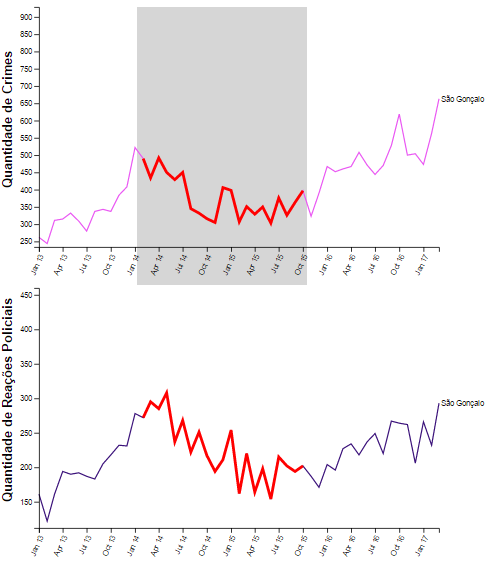
\includegraphics[width=3.5in]{relacaoRouboFurtoVeiculoRecuperacao.png}
% where an .eps filename suffix will be assumed under latex, 
% and a .pdf suffix will be assumed for pdflatex; or what has been declared
% via \DeclareGraphicsExtensions.
\caption{Histórico de roubos e furtos de veículos para os crimes e de recuperação de veículos para a ação policial.}
\label{fig_relacaoVeiculos}
\end{figure}

\section{Conclusão e trabalhos futuros}

Neste trabalho criamos uma ferramenta visual que permite a configuração de análises com dados de segurança em cidades. Através desta ferramenta buscamos extrair algum conhecimento não óbvio a partir dos dados de segurança do estado do Rio de Janeiro. 

Como a flexibilidade do sistema é grande e a quantidade de variáveis é alta optamos por analisar somente um sub-conjunto dos dados e parâmetros fixando outros. Análises mais aprofundadas podem ser efetuadas com a variação das configurações de forma direcionada com janelas de tempo, granularidades específicas e todos os demais parâmetros disponíveis.

Foram obtidos resultados não óbvios para alguns índices analisados como a presença de municípios do interior e região dos lagos nas primeiras posições relacionadas as altas taxas de crimes por habitante.  

Em trabalhos futuros iremos focar em casos específicos que envolvam configurações de pesos na criação dos índices de segurança para analisar o quanto esta opção pode auxiliar estes casos.

Outro aspecto é o aumento da escalabilidade do sistema, que pode ser obtida com a substituição da estrutura de dados (utilizada no dicionário) por um banco de dados.

Acreditamos ser importante buscar informações sobre número de policiais alocados por delegacia e por batalhão de forma a poder identificar superalocação ou subalocação policial por região analisada.

% conference papers do not normally have an appendix


% use section* for acknowledgment
\newif\ifacks
\acksfalse
%\acksltrue
\ifacks
\section*{Agradecimentos}
O autor R.H.C.M. agradece o suporte financeiro da CAPES. 
\fi

% trigger a \newpage just before the given reference
% number - used to balance the columns on the last page
% adjust value as needed - may need to be readjusted if
% the document is modified later
%\IEEEtriggeratref{8}
% The "triggered" command can be changed if desired:
%\IEEEtriggercmd{\enlargethispage{-5in}}

% references section

% can use a bibliography generated by BibTeX as a .bbl file
% BibTeX documentation can be easily obtained at:
% http://mirror.ctan.org/biblio/bibtex/contrib/doc/
% The IEEEtran BibTeX style support page is at:
% http://www.michaelshell.org/tex/ieeetran/bibtex/
\bibliographystyle{IEEEtran}
% argument is your BibTeX string definitions and bibliography database(s)
\bibliography{example}
%
% <OR> manually copy in the resultant .bbl file
% set second argument of \begin to the number of references
% (used to reserve space for the reference number labels box)
%\begin{thebibliography}{1}
%
%\bibitem{IEEEhowto:kopka}
%H.~Kopka and P.~W. Daly, \emph{A Guide to \LaTeX}, 3rd~ed.\hskip 1em plus
%  0.5em minus 0.4em\relax Harlow, England: Addison-Wesley, 1999.

%\end{thebibliography}




% that's all folks
\end{document}


